% -----------------------------------------------------------------------------
\begin{frame}[c]
\frametitle{Predictive control, operating WWTPs as self-sufficient WRRFs} \justifying

\boxHighlight[0.95\textwidth]{ \centering
    \textbf{Paradigm shift:} Wastewater as a sustainable source of water, energy, and raw materials
}

\vfill

\begin{center}
    \includegraphics<1>[width=0.95\textwidth]{figs/ControlFramework_01}%
    \includegraphics<2>[width=0.95\textwidth]{figs/ControlFramework_02}%
\end{center}

\vfill

\onslide<2>{
\boxInfo[0.95\textwidth]{\centering
    \textbf{Proposal $A$:} Predictive control to enable self-sufficient water resource recovery facilities
}
}

\end{frame}

% -----------------------------------------------------------------------------
\begin{frame}[t]
\frametitle{Predictive control, operating WWTPs as self-sufficient WRRFs (cont.)}\justifying
	
\vskip1em

\boxHighlight[0.9\textwidth]{ \centering
    We consider the task of operating a \textbf{biological wastewater treatment plant} (WWTP, secondary treatment) as a \textbf{water resource recovery facility} (WRRF)
}

\vskip1em

\begin{columns}
	\column[c]{0.45\textwidth}%
	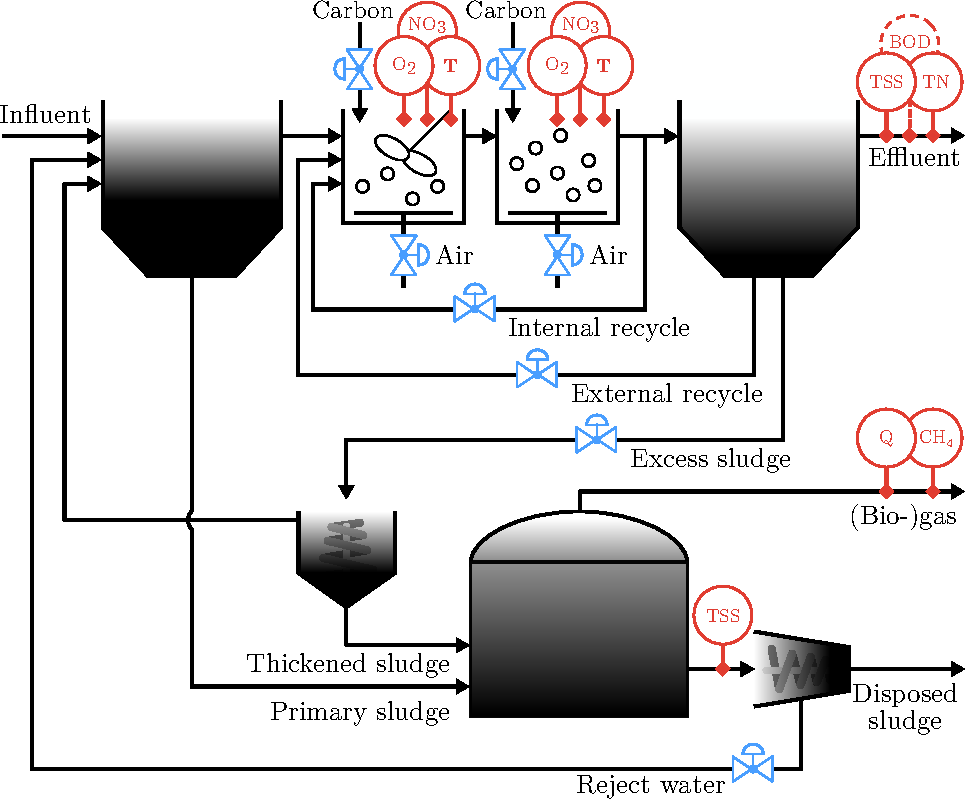
\includegraphics[width=\columnwidth]{figs/WRRF_Schematic_Instrumented_Colors}

	\column[c]{0.54\textwidth}
	\begin{itemize}
		\item {\color{monokaiOrange}\sc Primary objective:}\\
		on demand, produce effluent water of specific quality
		\vskip0.5em
		\begin{center}
            \begin{tabular}{@{}c ccc@{}} \toprule
                Water class & \multicolumn{3}{c}{Biochemical profile}                   \\\midrule
                            & {\small TSS}      &    {\small BOD}   &    {\small  TN}   \\\cmidrule{2-4}
                \textbf{A}  & $\leq 30$ g/m$^3$ & $\leq 10$ g/m$^3$ & $\leq 15$ g/m$^3$ \\
                \textbf{B}  & $\leq 30$ g/m$^3$ & $\leq 15$ g/m$^3$ & $\leq 30$ g/m$^3$ \\
                \textbf{C}  & $\leq 30$ g/m$^3$ & $\leq 20$ g/m$^3$ & $\leq 45$ g/m$^3$ \\\bottomrule
            \end{tabular}
		\end{center}
		\vskip1.5em
		%
		\item {\color{monokaiOrange}\sc Secondary objective:}\\
		produce biogas to ensure nonpositive energy cost index,
		\begin{multline*}
			\text{ECI} = \text{AE} + \text{PE} + \text{ME} - \eta_{E} \text{MP} \\
                            + \max(0, \text{HE} - \eta_{H}\text{MP})
		\end{multline*}
	\end{itemize}
\end{columns}

\end{frame}

%------------------------------------------------------- 
\begin{frame}[t]
\frametitle{Predictive control, general architecture and specific configuration}\justifying

\vfill
\begin{columns}
	\column[t]{0.5\textwidth}
	\begin{center}
		\vskip-1.5em
		\includegraphics<1>[width=0.98\columnwidth]{figs/Control_Diagram_Isolated}% 
		\includegraphics<2>[width=0.98\columnwidth]{figs/Control_Diagram_Isolated_H1}% 
		\includegraphics<3>[width=0.98\columnwidth]{figs/Control_Diagram_Isolated_H2}% 
		\includegraphics<4>[width=0.98\columnwidth]{figs/Control_Diagram_Isolated_H3}% 
	\end{center}

	\column[t]{0.49\textwidth}
	We design a \textbf{model-based} output-feedback controller
	\begin{align*}
		\textstyle\frac{d}{dt}\clX{x(t)} &= f(\clX{x(t)}, \clU{u(t)}, \clW{w(t)}) & {\color{gray}(dynamics)} \\
		\clY{y(t)}   				     &= g(\clX{x(t)}, \clU{u(t)})			  & {\color{gray}(measurements)} \\
		\clY{z(t)}   				     &= h(\clX{x(t)}, \clU{u(t)})			  & {\color{gray}(performance)}
	\end{align*}

	\vskip0.5em
	which autonomously operates the plant in cycles	
	\begin{center}
		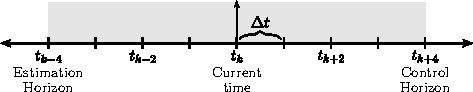
\includegraphics[width=0.95\columnwidth]{figs/Control_Diagram_Time}
	\end{center}
\end{columns}

\vfill
\only<1>{\vskip6.5em}%
\only<2->{\centering%
\begin{columns}
	\column{0.01\textwidth} \,
	\column<2->{0.28\textwidth}
	\begin{block}{\sc Operating point optimiser} \centering
		Determines an \textit{\color{stateColor}operating point} which yields the \textit{\color{outputColor}desired key performance indicators}
	\end{block}

	\column{0.03\textwidth} \centering
	$$\Longrightarrow$$

	\column<3->{0.28\textwidth}
	\begin{block}{\sc Moving horizon estimator} \centering
		Determines an \textit{\color{stateColor}estimate of the current state} based on \textit{\color{outputColor}measurement data}
	\end{block}

	\column{0.03\textwidth} \centering
	$$\Longrightarrow$$

	\column<4->{0.28\textwidth}
	\begin{block}{\sc Model predictive control} \centering
		Determines a \textit{\color{inputColor}sequence of control actions} to regulate the plant to the \textit{\color{stateColor}operating point}
	\end{block}
		
	\column{0.01\textwidth} \,
\end{columns}
}

\end{frame}
	
%------------------------------------------------------- 
\begin{frame}[c]
\frametitle{Predictive control, experimental results}\justifying

\only<3>{
\boxInfo[0.85\textwidth]{ \centering
    (On average) the controller renders the WRRF energetically self-sufficient
}
\vskip2em
}

\begin{center}
	\only<1>{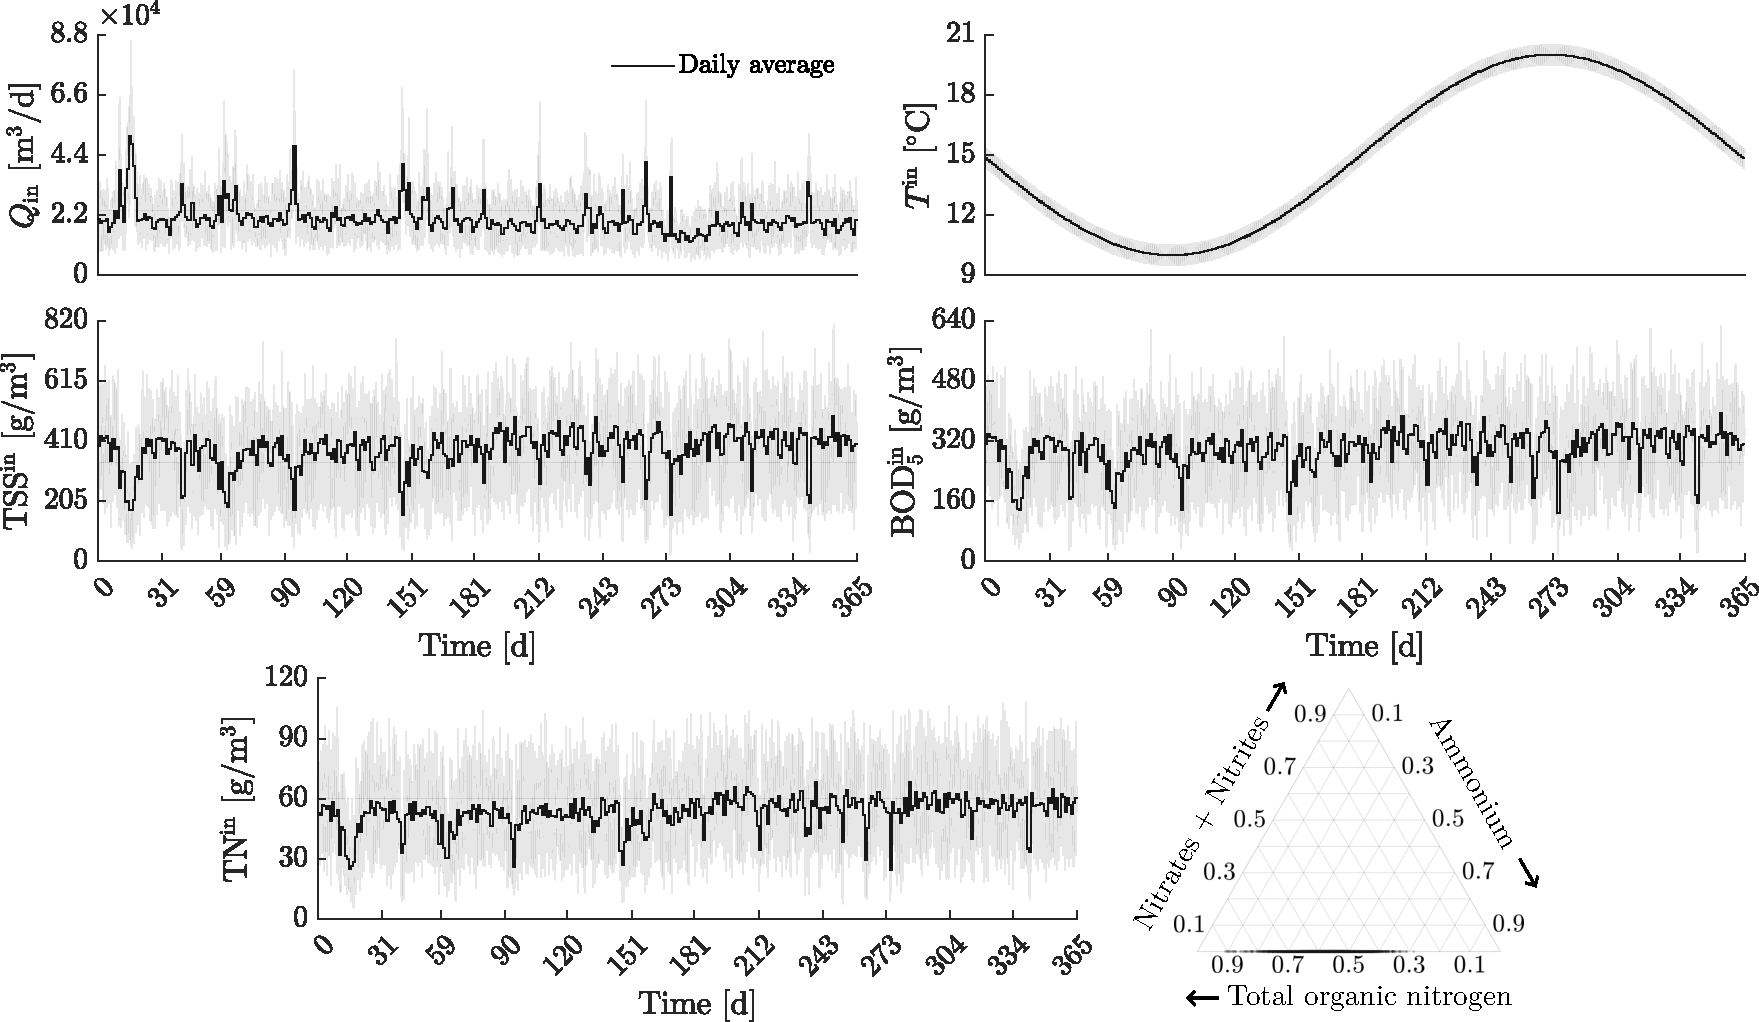
\includegraphics[width=0.9\textwidth]{figs/Simulation_Influent}}%
	\only<2>{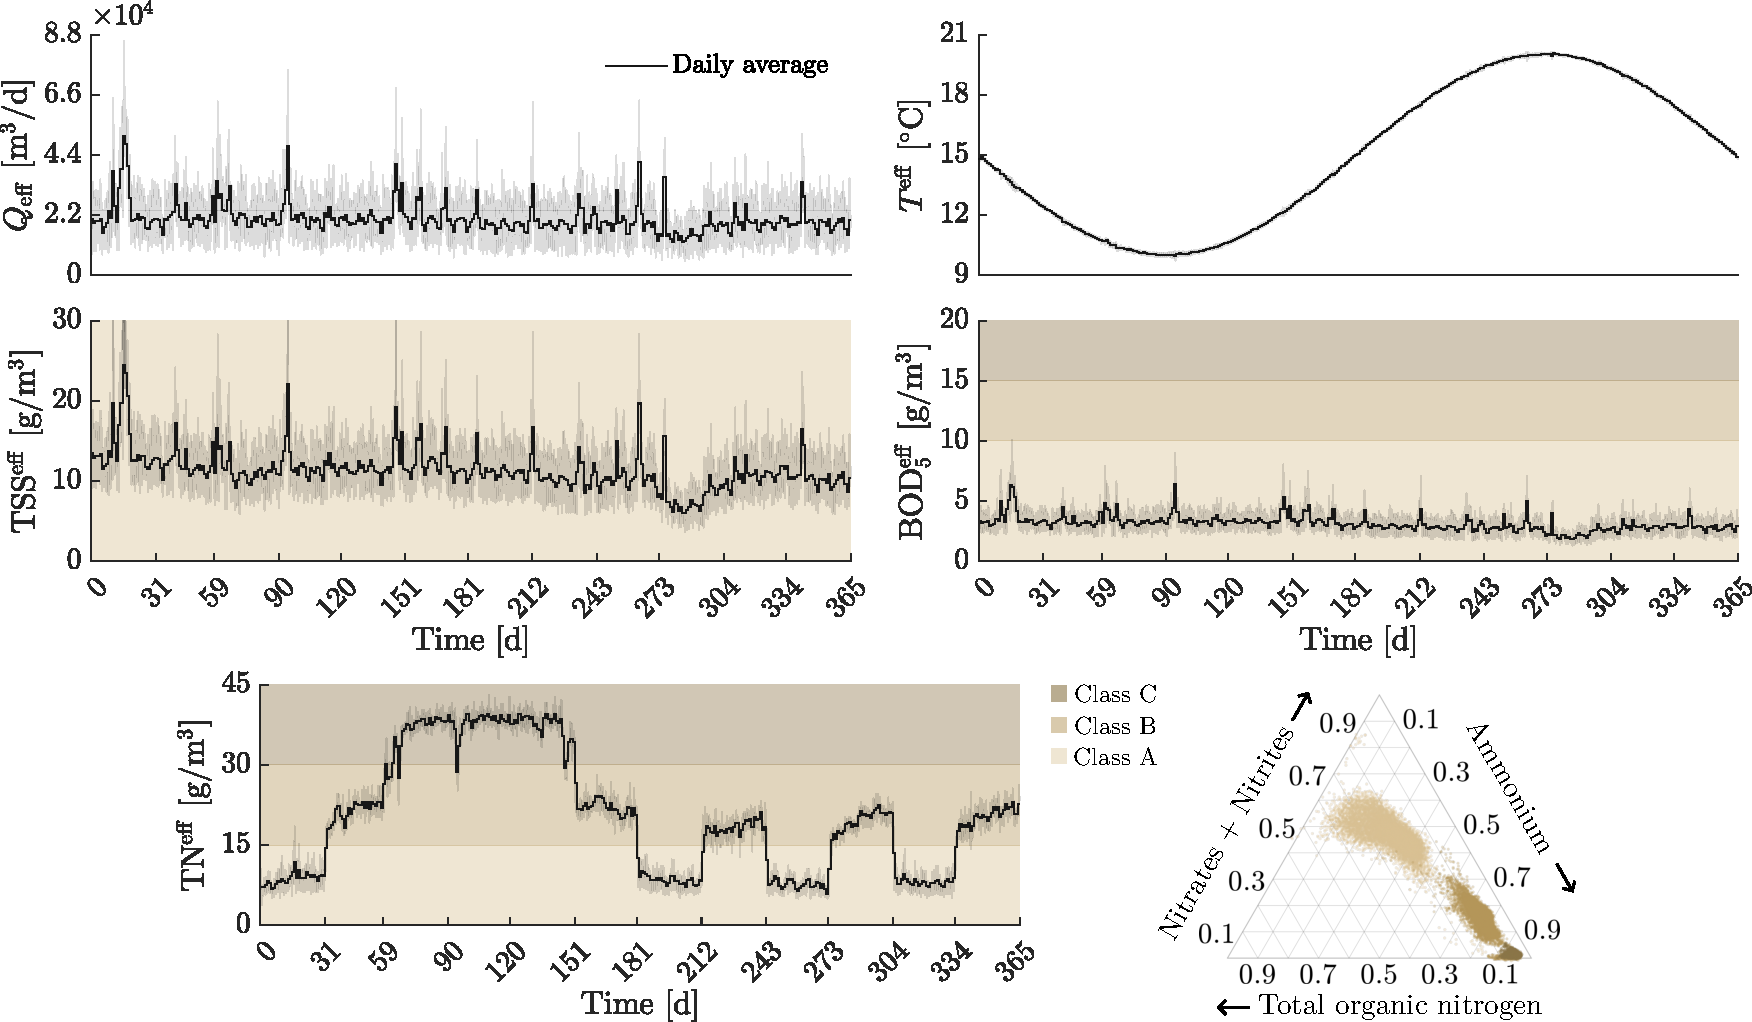
\includegraphics[width=0.9\textwidth]{figs/Simulation_Effluent}}%
	\only<3>{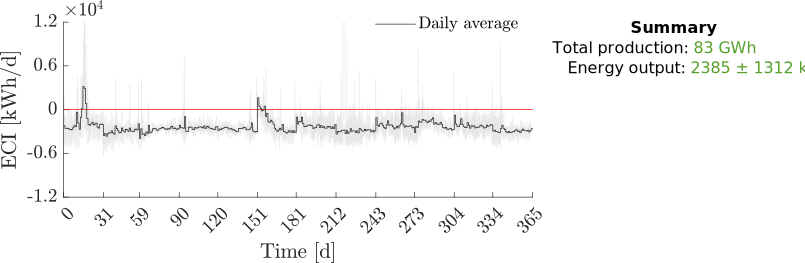
\includegraphics[width=0.85\textwidth]{figs/Simulation_ECI}}%
\end{center}

\end{frame}
%------------------------------------------------------- 
